\documentclass{article}
%% Useful packages
\usepackage[utf8]{inputenc}
\usepackage[a4paper,left=2cm,right=2cm,top=2cm,bottom=2cm]{geometry}
\usepackage{crop,graphicx,amsmath,array,color,amssymb,fancyhdr,lineno}
\usepackage{flushend,stfloats,amsthm,chngpage,times,,lipsum,lastpage} 
\usepackage{calc,listings,color,wrapfig,tabularx,longtable,enumitem}
\usepackage[style=numeric-comp,backend=biber]{biblatex}
\addbibresource{Refs.bib}
\usepackage{lineno}
%%%%%%%%%%%%   Header and Footer  %%%%%%%%%%%%%
\pagestyle{fancy}
\fancypagestyle{plain}{%
  \renewcommand{\headrulewidth}{0pt}%
  \fancyhf{}%
}

\title{%
  First Assignment \\
  \large Equivalent representations of orientation matrices}
\author{Surname Name}

\begin{document}
\begin{titlepage}

\newcommand{\HRule}{\rule{\linewidth}{0.5mm}} % Defines a new command for the horizontal lines, change thickness here

%----------------------------------------------------------------------------------------
%	LOGO SECTION
%----------------------------------------------------------------------------------------
\center

\includegraphics[width=5cm]{Title/Unige-logo.jpeg}\\[1cm] % Include a department/university logo - this will require the graphicx package
 
%----------------------------------------------------------------------------------------

\center % Center everything on the page

%----------------------------------------------------------------------------------------
%	HEADING SECTIONS
%----------------------------------------------------------------------------------------

\textsc{\Huge Università degli studi di Genova}\\[1cm] % Name of your university/college
\textsc{\LARGE DIBRIS}\\[0.3cm]
\textsc{\Small Department of Computer Science and Technology,}\\
\textsc{\Small Bioengineering, Robotics and System Engineering}\\[1cm] % Minor heading such as course title
\textsc{\LARGE{Modelling and Control of Manipulators}}\\[1cm] % Major heading such as course name

%----------------------------------------------------------------------------------------
%	TITLE SECTION
%----------------------------------------------------------------------------------------
\makeatletter
\HRule \\[0.4cm]
{ \huge \bfseries Second Assignment}\\[0.2cm] 
{\Large \bfseries Manipulator Geometry and Direct Kinematics}\\
% Title of your document
\HRule \\[1.5cm]
 
%----------------------------------------------------------------------------------------
%	AUTHOR SECTION
%----------------------------------------------------------------------------------------

\begin{minipage}{0.4\textwidth}
\begin{flushleft} \large
\emph{Author:}\\[0.2cm]
Surname Name % Your name
\\[1.2em]
\emph{Student ID:}\\[0.2cm]
s0000000 \\[1.2em]
\end{flushleft}
\end{minipage}
~
\begin{minipage}{0.4\textwidth}
\begin{flushright} \large
\emph{Professors:} \\[0.2cm]
Enrico Simetti\\
Giorgio Cannata  \\[1.2em] % Supervisor's Name

\emph{Tutors:} \\[0.2cm]
Andrea Tiranti\\
Luca Tarasi\\
George Kurshakov
% second marker's name
\end{flushright}
\end{minipage}\\[2cm]
\makeatother

% If you don't want a supervisor, uncomment the two lines below and remove the section above
%\Large \emph{Author:}\\
%John \textsc{Smith}\\[3cm] % Your name

%----------------------------------------------------------------------------------------
%	DATE SECTION
%----------------------------------------------------------------------------------------

{\large \today}\\[2cm] % Date, change the \today to a set date if you want to be precise

\vfill % Fill the rest of the page with whitespace

\end{titlepage}

\sffamily

\fancyhf{}
\fancyhead[L]{Surname Name - s0000000}
\fancyhead[R]{Modelling and Control of Manipulators - Assignment 2}
\fancyfoot[R]{ \bf\thepage\ \rm }%

\newpage
\tableofcontents

\section*{}
\begin{longtable}{|p{4cm}|p{4cm}|p{4cm}|}
    \hline
    Mathematical expression & Definition & MATLAB expression \\
    \hline 
    $<w>$ & World Coordinate Frame &  w\\[0.4cm]
    $^a_b R$ & Rotation matrix of frame $<b>$ with respect to frame $<a>$  & aRb \\[1.2cm]
    $^a_b T$ & Transformation matrix of frame $<b>$ with respect to frame $<a>$ & aTb \\[1.2cm]
    \hline
    \caption{Nomenclature Table}
\end{longtable}

\section{Assignment description}
The second assignment of Modelling and Control of Manipulators focuses on manipulators' geometry and direct kinematics. 

\begin{itemize}
    \item Download the .zip file called \textit{template\_MATLAB-assignment2} from the Aulaweb page of this course.
    \item Implement the code to solve the exercises on MATLAB by filling the template classes called \textit{geometricModel} and \textit{kinematicModel}
    \item Write a report motivating your answers, following the predefined format on this document.
\end{itemize}

\subsection{Exercise 1}
 Given the following CAD model of an industrial 7 DoF manipulator:
 
\textbf{Q1.1} Define all the model matrices, by filling the structures in the \textit{BuildTree()} function. Be careful to define the z-axis coinciding with the joint rotation axis, and such that the positive rotation is the same as showed in the CAD model you received. Draw on the CAD model the reference frames for each link and insert it into the report.

\textbf{Q1.2} Implement the method of \textit{geometricModel} called \textit{updateDirectGeometry()} which should compute the model matrices as a function of the joint position $q$. Explain the method used and comment on the results obtained.

\textbf{Q1.3} Implement the method of \textit{geometricModel} called \textit{getTransformWrtBase()} which should compute the transformation matrix from the base to a given frame. Calculate the following transformation matrices: $^b_e T$, $^5_3 T$. Explain the method used and comment on the results obtained.

\textbf{Q1.4} Implement the method of \textit{kinematicModel} called \textit{updateJacobian()} which should compute the jacobian of a given geometric model considering the possibility of having \textit{rotational} or \textit{prismatic} joints. Compute the Jacobian matrix of the manipulator for the end-effector. Explain the method used and comment on the results obtained.

\textit{Remark:} The methods should be implemented for a generic serial manipulator. For instance, joint types, and the number of joints should be parameters. 

\newpage

\begin{figure} [ht]
\centering
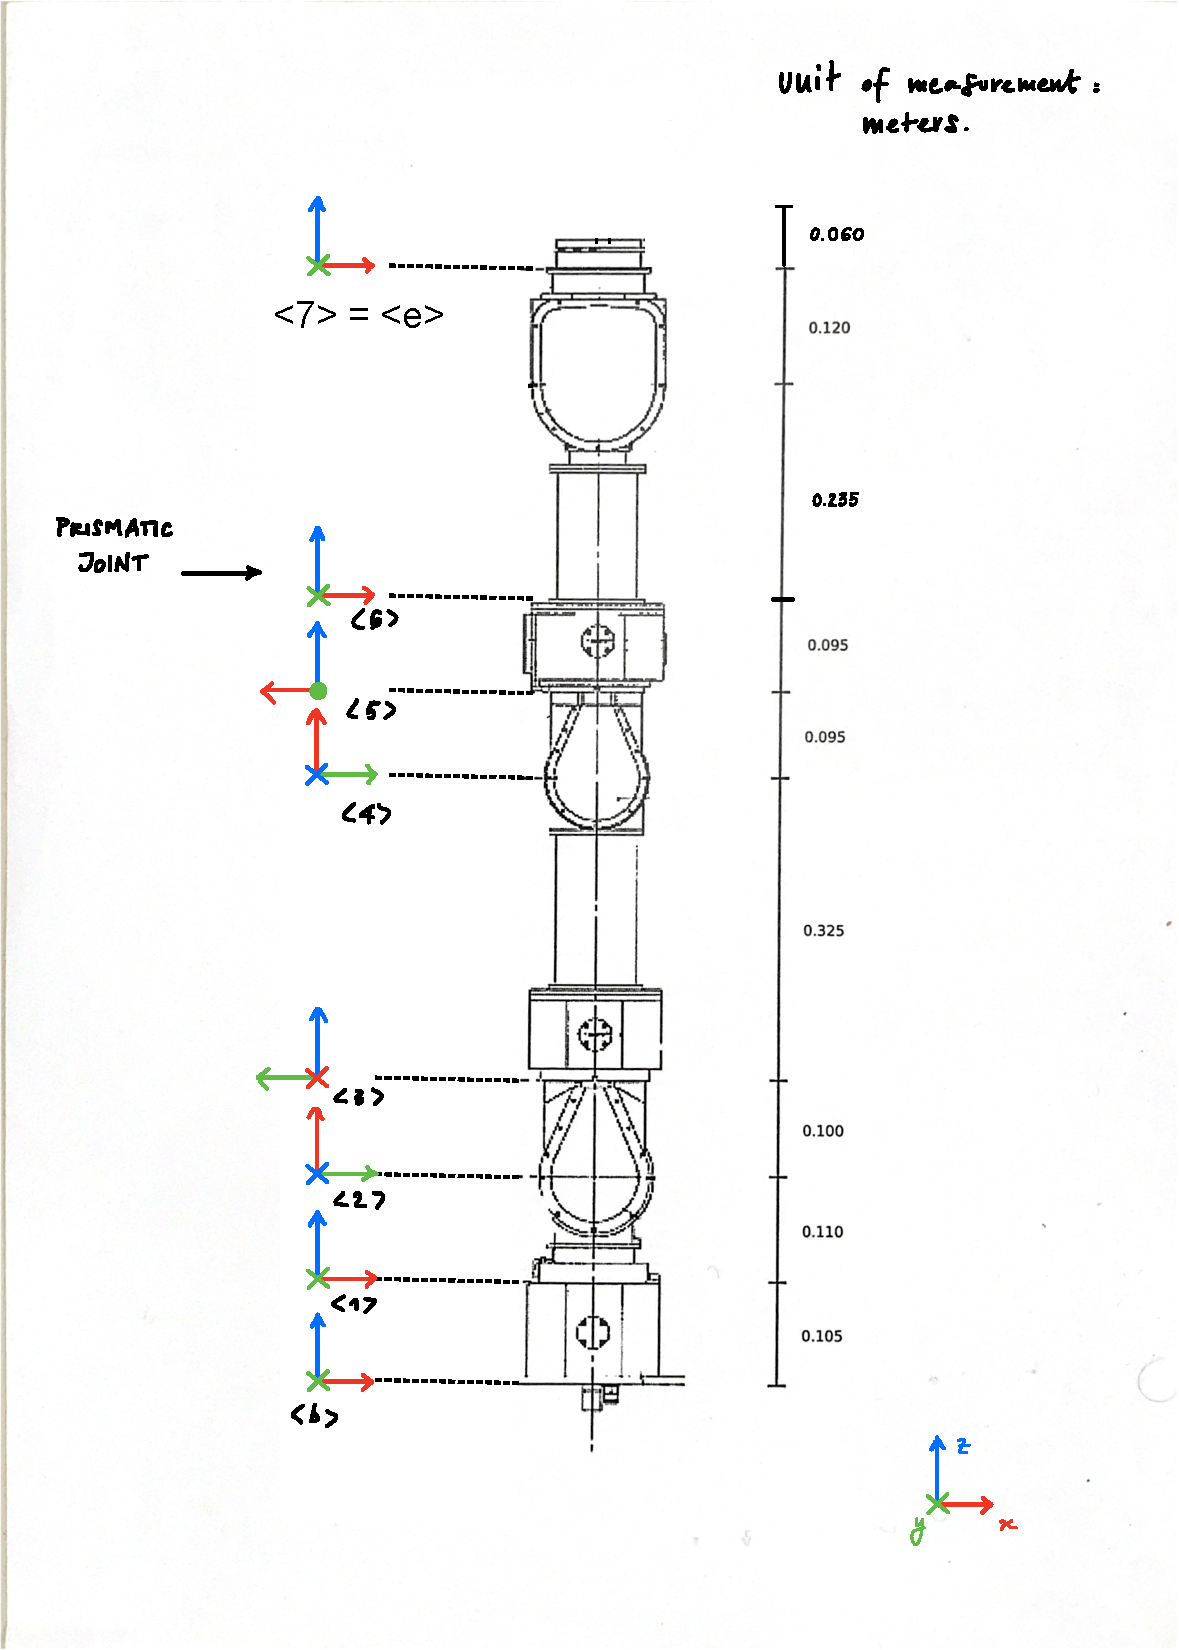
\includegraphics[width=\textwidth*8/10]{Resources/cad_model-1.pdf}
\caption{CAD model of the robot}
\label{fig:ex2}
\end{figure}

\newpage
\section{Exercise 1} \label{P1}
% Write some intro
\textit{[Comment] For the last exercises include an image of the initial robot image of the final robot configuration} 

\textit{[Comment] For each exercise report the results obtained and provide an explanation of the result obtained (even though it might seem trivial). The matlab code is NOT an explanation of the algorithm.} 

\pagebreak

\section{Appendix}
\textit{[Comment] Add here additional material (if needed)} 
\subsection{Appendix A}

\subsection{Appendix B}


\end{document}
